% !TeX root = ../sustechthesis-example.tex

\chapter{弹性杆模型及细长结构稳定性分析}

\section{引言}

建立弹性蛇形条带结构的力学模型是研究其分岔行为和进行结构稳定性分析的基础。由于其细长的几何特性,蛇形条带的弯曲和扭转刚度较低,在外载荷作用下,在满足小应变假设(即线弹性本构关系)的前提下,结构仍会产生较大的位移变形。因此,本文采用基于线性本构关系的弹性杆模型,并考虑结构的几何非线性效应。具体而言,本文主要采用两种弹性杆模型:离散弹性杆模型和基尔霍夫杆弹性杆模型。

离散弹性杆模型中考虑了惯性力,属于动力学模型。因此利用该模型,不仅可以求得结构在给定载荷作用下的平衡解,而且可以利用线性化的动力学稳定性判据来判断平衡解的稳定性;而基尔霍夫杆模型是经典的静力学弹性杆模型,由于该模型为不可拉伸杆模型,更加符合细长杆的建模,因而能给出更为精确的解,但该模型无法直接对所得解的稳定性进行判定。因此,本文结合了两套模型的优势:利用基尔霍夫杆模型进行分岔分析以获得更精确的解,同时利用离散弹性杆模型通过动力学稳定性判定方法对所得解的稳定性进行判断。另外,在后续研究蛇形结构多稳态行为时,仍需要利用动力学模态来寻找稳态解。

本章首先系统介绍离散弹性杆模型与基尔霍夫杆模型的理论框架。随后,详细阐述本文用于分析结构后屈曲行为的主要方法与工具——参数延拓法,以及用于结构稳定性判定的理论依据。最后,通过对典型结构的计算分析,验证基于线性化的动力学稳定性判据在判定平衡解稳定性方面的有效性。

\section{基尔霍夫杆模型}
\subsection{标架运动学方程}
根据微分几何的曲线论基本定理可知,任意一条空间曲线的构形可以由该曲线在任意弧长处的曲率和挠率两个量完全确定。在刻画一条空间曲线的构形时,通常会在任意弧长处定义一个Frenet标架,该标架的第三个坐标轴与曲线相切;第一个坐标轴指向曲线的弯曲方向,即与$d\overrightarrow{\mathbfit{t}}/\dif s$共线,其中$\overrightarrow{\mathbfit{t}}$为曲线的单位切向量,称为主法向量;第二个坐标轴与其他两个坐标轴共同构成构成右手坐标系,称为次法向量。

而为了确定一根细长弹性杆的空间构形,不仅仅需要确定中心线的空间位置,还需确定任意弧长处弹性杆截面的空间取向。细长弹性杆的几何构形通常可以用一条框架曲线来刻画,如图~\ref{fig:Material Frame}所示。红色虚线为弹性杆的中心线,并且在该曲线的任意弧长处附有一材料标架用来刻画细长弹性杆截面的空间方位。该标架的原点在中心线上,三个坐标轴分别与曲线的切线$\mathbfit{t}$以及弹性杆截面的两个主惯性轴$\mathbfit{d}_1,\mathbfit{d}_2$共线。因此,一根弹性杆可以由三个量来确定:任意弧长处的曲率,挠率,以及材料标架与Frenet标架绕共同切线轴的相对转角。
\begin{figure}
	\centering
	\includegraphics[width=0.8\linewidth]{Material frame.pdf}
	\caption{细长杆变形前后相应的框架曲线}
	\label{fig:Material Frame}
\end{figure}

下面给出材料标架的沿弧长的运动学关系,由于材料标架三个轴总保持互相垂直,因此材料标架对弧长$s$的导数满足
    \begin{equation}
    \centering
	\mathbfit{d}'_{\alpha}=\mathbfit{\Omega}\times\mathbfit{d}_{\alpha},\quad
	\mathbfit{\Omega}=\mathbfit{t}\times \mathbfit{t}'+m \mathbfit{t}   
    \label{eq:Darboux vector}
    \end{equation}
式中下标$\alpha$可以取$1$,$2$,$3$分别对应材料标架的三个坐标轴,这里$\mathbfit{d}_3$轴为$\mathbfit{t}$轴。$\mathbfit{\Omega}$称为Darboux向量,该向量用来刻画材料标架沿弧长的变化率,可以分两部分:第一部分为$\kappa \mathbfit{b}=\mathbfit{t}\times \mathbfit{t}'$,该项保证了材料标架沿弧长变化过程中坐标轴$\mathbfit{t}$总是与中心线相切;第二部分中$m=\mathbfit{d}'_1 \cdot \mathbfit{d}'_2$,该项用来刻画材料标架沿弧长绕切线轴转动的变化率。

在实际计算过程中,为了避免由于欧拉角的引入而产生可能的数值奇异,本文采用四元数来刻画材料标架随弧长的转动,设Darboux向量$\mathbfit{\Omega}=\kappa_1\mathbfit{d}_1+\kappa_2\mathbfit{d}_2+\tau \mathbfit{t}$,四元数为$\mathbfit{q}=(q_1,q_2,q_3,q_4)$,Darboux向量与四元数导数的关系如式\eqref{eq:Derivative of Quaternion}所示
\begin{equation}
	\centering 
	\begin{split}
    &q_1'=\frac{1}{2}(-\kappa_1 q_2-\kappa_2 q_3-\tau q_4) \\
    &q_2'=\frac{1}{2}(\kappa_1 q_1+\tau q_3-\kappa_2 q_4) \\
    &q_3'=\frac{1}{2}(\kappa_2 q_1-\tau q_2+\kappa_1 q_4) \\
    &q_4'=\frac{1}{2}(\tau q_1+\kappa_2 q_2-\kappa_1 q_3) \\
\end{split}
	\label{eq:Derivative of Quaternion}
\end{equation}


\subsection{平衡方程及本构关系}
本小节将通过微元法来推导细长弹性杆的平衡方程并给出本构关系。
\begin{figure}
	\centering
	\includegraphics[width=0.5\linewidth]{equilibrium equation.pdf}
	\caption{弹性杆微元的受力图,$\mathbfit{F}$,$\mathbfit{M}$为截面上所受力与力矩,$\mathbfit{p}$,$\mathbfit{q}$为微元上分布力与分布力矩\cite{audoly2000elasticity}}
	\label{fig:Equilibrium equation}
\end{figure}
图~\ref{fig:Equilibrium equation}为弹性杆微元的受力分图,根据受力图,易得力平衡方程及力矩平衡方程,分别为
\begin{equation}
	\centering
	\begin{gathered}
		\mathbfit{F}(s+\dif s)-\mathbfit{F}(s)+\mathbfit{p}\dif s=0 \\
		\mathbfit{M}(s+\dif s)-\mathbfit{M}(s)
		+(\mathbfit{d}\mathbfit{r}/2)\times\mathbfit{F}(s+\mathbfit{d}s)
		-\mathbfit{dr}/2\times(-\mathbfit{F}(s))
		+\mathbfit{q}\dif s=0	
	\end{gathered}   
	\label{eq:Equilibrium equation}
\end{equation}
式中,$\mathbfit{F}$为作用在截面上的内力,$\mathbfit{p}$为作用在微元上的分布力,$\mathbfit{M}$为作用在截面上的内力矩,$\mathbfit{q}$为分布力矩。其中力矩平衡方程是关于点$A$的力矩平衡方程。将式\eqref{eq:Equilibrium equation}两端同时除以微元长度$\dif s$并忽略高阶项得
\begin{equation}
	\begin{split}
		&\mathbfit{F}'(s)+\mathbfit{p}(s)=0 \\
		&\mathbfit{M}'(s)
		+\mathbfit{d}_3(s)\times\mathbfit{F}(s)
		+\mathbfit{q}(s)=0	
	\end{split}   
	\label{eq:Equilibrium equation1}
\end{equation}

下面将介绍基尔霍夫杆的本构关系。该本构关系仅在小应变假设成立的条件下适用,即细长杆变形后曲率半径$R$远远大于细长杆截面的特征长度$h$的情况($R>>h$)下适用,本文所研究的结构该假设总成立。基尔霍夫杆的本构关系为线性关系,设Darboux向量为$\mathbfit{\Omega}=\kappa_1\mathbfit{d}_1+\kappa_2\mathbfit{d}_2+\tau \mathbfit{t}$,则该本构关系的具体表达式为式如\eqref{eq:Constitutive Law}所示
\begin{equation}
	\begin{split}
		&\mathbfit{M}(s)=G^{(1)}(s)\mathbfit{d}_1(s)+G^{(2)}(s)\mathbfit{d}_2(s)+H(s)\mathbfit{t}(s) \\
		 &G^{(1)}(s)=EI^{(1)}(\kappa_1(s)-\kappa_{10}(s))\\ 
		&G^{(2)}(s)=EI^{(2)}(\kappa_2(s)-\kappa_{20}(s))\\
		 &H(s)=G J\tau(s)	
	\end{split}   
	\label{eq:Constitutive Law}
\end{equation}
式中,$\kappa_{10}(s)$,$\kappa_{20}(s)$为弹性杆的初始曲率,$EI^{(1)}$,$EI^{(2)}$分别为绕主惯性轴$d_1$,$d_2$的弯曲刚度,$G J$为弹性杆的扭转刚度。
其中$E$为弹性模量,$G$为剪切弹性模量$G=E/2(1+\nu)$,$J$为极惯性矩,$\nu$为泊松比,本文中泊松比设为$0.33$。本文所研究的结构均为具有矩形截面形状的条带结构,这里给出矩形截面的条带结构的弯曲刚度与扭转刚度的具体表达式~\cite{timoshenko1969theory}:
\begin{equation}
	\begin{gathered}
  EI=\frac{1}{12}Ewt^3,\quad EI=\frac{1}{12}Ew^3t,\quad G J=\lambda w\frac{E}{2(1+\nu)}t^3 \\
  \lambda=\frac{1}{3}\left(1-\frac{192}{\pi^5}\frac{t}{w}\sum_{k=1}^{\infty}\frac{1}{(2k-1)^5}\tanh\left(\frac{\pi(2k-1)w}{2t}\right)\right)
  \end{gathered}
\end{equation}
式中,$w$,$t$分别为弹性杆截面的宽度和厚度。另外,拉伸刚度为$Ewt$,其量级为$o(h^2)$,$h$为截面特征长度。而弯曲刚度与扭转刚度的量级为为$o(h^4)$。由于特征长度$h$为小量,弹性杆的拉伸刚度远大于弯曲扭转刚度,因此基尔霍夫杆模型中,忽略拉伸引起的应变及相应的应变能,即基尔霍夫杆为不可拉伸杆。

在实际的计算过程中,需要将矢量方程表达为标量分量形式。由于上述给出的本构关系表达式是在局部材料标架下的投影形式,因此,为了方便本构关系的表达,这里选择将平衡方程同样在局部材料坐标系下投影,力的平衡关系式如下:
\begin{equation}
	\begin{split}
	&N_{1}^{\prime}=N_{2} \tau-N_{3} \kappa_{2}\\
	&N_{2}^{\prime}=-N_{1} \tau+N_{3} \kappa_{1}\\
	&N_{3}^{\prime}=-N_{2} \kappa_{1}+N_{1} \kappa_{2}
	\end{split}
\end{equation}
式中 $N_1$,$N_2$,$N_3$分别为弹性杆截面内力$\mathbfit{F}$在材料标架$\mathbfit{d_1}$,$\mathbfit{d_2}$,$\mathbfit{t}$下的分量。力矩平衡方程的分量表达式为
\begin{equation}
	\begin{split}
	&\frac{\mathrm{d} G^{(1)}}{\mathrm{d} s}-G^{(2)} \tau+H \kappa^{(2)}-N_{2}+q_{1}=0 \\
	&\frac{\mathrm{d} G^{(2)}}{\mathrm{d} s}-H \kappa^{(1)}+G^{(1)} \tau+N_{1}+q_{2}=0 \\
	&\frac{\mathrm{d} H}{\mathrm{d} s}-G^{(1)} \kappa^{(2)}+G^{(2)} \kappa^{(1)}+q_{3}=0
	\end{split}
\end{equation}
式中$q_{1}$,$q_{2}$,$q_{3}$分别为分布力矩在材料标架$\mathbfit{d_1}$,$\mathbfit{d_2}$,$\mathbfit{t}$下的分量。本处需要强调,在表达力与力矩的分量时,由于材料标架不是固定标架而是沿弧长变化的标架,因此在求导数时,应当考虑标架本身的导数,即	$\mathbfit{d}'_{\alpha}=\mathbfit{\Omega}\times\mathbfit{d}_{\alpha}$。
\subsection{边界值问题的构造}
为了求解给定细长结构在外载荷下的非线性行为,需要将该力学问题构造为一个适定的边界值问题。前几小节中,给出了细长弹性杆力与力矩的平衡方程,材料标架的运动方程。此外,为了得到弹性杆中心线的位置,需要通过对切向量沿弧长进行积分,若规定材料标架的切向量对应于全局坐标系的$Z$轴$(0,0,1)$,中心线位置与切向量的微分关系为
\begin{equation}
	\begin{split}
	&x^{\prime}=2\left(q_{2} q_{4}+q_{1} q_{3}\right)\\ 
	&y^{\prime}=2\left(q_{3} q_{4}-q_{1} q_{2}\right)\\ 
	&z^{\prime}=2\left(q_{1}^{2}+q_{4}^{2}-\frac{1}{2}\right)
	\end{split}
\end{equation}
若切向量不与全局坐标系的$Z$轴对应,可通过关系式\eqref{eq:the different compoments in different frames}得到中心线的位置。
\begin{equation}
	\mathbfit{t}=\mathbfit{R}_q(\mathbfit{q})^{\top}\mathbfit{t}^{(1)}
	\label{eq:the different compoments in different frames}
\end{equation}
式中$\mathbfit{t}$,$\mathbfit{t}^{(1)}$分别为曲线切向量在全局坐标系和材料标架下的分量,$\mathbfit{R}_q(\mathbfit{q})$为以四元数表示的全局坐标系与材料标架之间的旋转矩阵\cite{henderson1977euler},具体如下:
\begin{equation}
	\mathbfit{R}_{q}(\mathbfit{q})= 2\left[\begin{array}{ccc}q_{1}^{2}+q_{2}^{2}-\frac{1}{2} &  q_{2} q_{3}+ q_{1} q_{4} &  q_{2} q_{4}- q_{1} q_{3} \\ q_{2} q_{3}- q_{1} q_{4} & q_{1}^{2}+q_{3}^{2}-\frac{1}{2} &  q_{3} q_{4}+ q_{1} q_{2} \\ q_{2} q_{4}+ q_{1} q_{3} &  q_{3} q_{4}- q_{1} q_{2} & q_{1}^{2}+q_{4}^{2}-\frac{1}{2}\end{array}\right] 
		\label{eq:Rotation Matrix}
\end{equation}

在实际计算中,将弹性杆长度进行归一化处理,若弹性杆长度为$l$,$s\in(0,l)$,为了进行归一化处理,这里将方程中变量替换为$s$替换为$\overline sl$,$\overline s\in(0,1)$。在变量替换过程中为了保持原方程不变,对于导数项则需要利用链式法则进行求导,首先对$\overline s$求导,随后将$\overline s$对$s$求导得$1/l$。以变量$\mathrm{d}N_1(s)/\mathrm{d}s$为例,变量替换后该项应为$\mathrm{d}N_1(\overline s)/\mathrm{d}\overline{s}/l$。

综上所示,为了求解计算细长弹性杆的分岔行为,前几小结给出了13个方程,分别为三个力平衡方程,三个力矩平衡方程(带入本构关系,用Darboux向量来表示该平衡方程),四个由四元数表示的材料标架的运动方程,以及三个表示中心线位置与切向量关系的方程。设一弹性杆的长度为$l$,截面形状为矩形,那么相应的微分方程总结如下,
\begin{equation}
	\begin{split}
	&N_{1}^{\prime}=(N_{2} \tau-N_{3} \kappa_{2})l\\
	&N_{2}^{\prime}=(-N_{1} \tau+N_{3} \kappa_{1})l \\
	&N_{3}^{\prime}=(-N_{2} \kappa_{1}+N_{1} \kappa_{2})l \\
	&a \kappa_{1}^{\prime}=(b\left(\kappa_{2}-\kappa_{20}\right) \tau-\tau \kappa_{2}+N_{2})l \\
	&b \kappa_{2}^{\prime}=(-a (\kappa_{1}-\kappa_{10}) \tau+\tau \kappa_{1}-N_{1})l \\\
	&\tau^{\prime}=(-b\left(\kappa_{2}-\kappa_{20}\right) \kappa_{1}+a (\kappa_{1}-\kappa_{10}) \kappa_{2})l \\ 
	&q_{1}^{\prime}=\frac{1}{2}\left(-q_{2} \kappa_{1}-q_{3} \kappa_{2}-q_{4} \tau\right)l+\mu q_{1}l\\
	&q_{2}^{\prime}=\frac{1}{2}\left(q_{1} \kappa_{1}-q_{4} \kappa_{2}+q_{3} \tau\right)l+\mu q_{2}l\\ 
	&q_{3}^{\prime}=\frac{1}{2}\left(q_{4} \kappa_{1}+q_{1} \kappa_{2}-q_{2} \tau\right)l+\mu q_{3}l\\ 
	&q_{4}^{\prime}=\frac{1}{2}\left(-q_{3} \kappa_{1}+q_{2} \kappa_{2}+q_{1} \tau\right)l+\mu q_{4}l \\
	&x^{\prime}=2\left(q_{2} q_{4}+q_{1} q_{3}\right)l\\
	&y^{\prime}=2\left(q_{3} q_{4}-q_{1} q_{2}\right))l\\
	&z^{\prime}=2\left(q_{1}^{2}+q_{4}^{2}-\frac{1}{2}\right)l\\
    &\mu^{\prime}=0
	\end{split}
	\label{eq:ToTle Equation}
\end{equation}
式中, $a$,$b$分别为无量纲化后的两个主惯性轴方向的弯曲刚度。将细长弹性杆的扭转刚度设为1,作为单位来对弯曲刚度进行无量纲化。具体表达式如下
\begin{equation}
	a=\frac{E I_{1}}{G J}=\frac{(1+v)}{6 \lambda}, b=\frac{E I_{2}}{G J}=\frac{(1+v)}{6 \lambda}\left(\frac{w}{t}\right)^{2}
\end{equation}

为了求解细长弹性杆的非线性行为,除了给定结构的控制方程外,还有需要给定相应的边界条件。本文所讨论的主要结构为蛇形条带,其边界条件为两端固支边界条件。由初始端($s=0$)固支条件可以给出七个边界条件,即初始端的位置向量以及由四元数给出的初始端截面空间取向。同理,在末端处($s=1$)可以施加同样的七个边界条件,总共构成$14$个边界条件,而方程个数为$13$。这种方程个数与边界条件个数不匹配的原因是由于四元数四个分量之间并非相互独立,存在下述约束关系式
\begin{equation}
	{q_1}^2+{q_2}^2+{q_3}^2+{q_4}^2=1
	\label{eq:constraint term}
\end{equation}

为了解决方程个数与边界条件个数不匹配的问题,本文采用Healey~\cite{healey2005straightforward}所提出的方法,通过引入常变量$\mu$来解决方程适定性的问题。对于变量之间存在代数约束的微分方程
\begin{equation}
	\begin{split}
	&\dot{\mathbfit{x}}=\mathbfit{f}(\mathbfit{x})\\
	&E(\mathbfit{x})\equiv C
	\end{split}
	\end{equation}
可以通过引入常变量$\mu$来构造一个增广系统
\begin{equation}
		\dot{\mathbfit{x}}=\mathbfit{f}(\mathbfit{x})+\mu \nabla E(\mathbfit{x}), \quad a<t<b
\end{equation}
若方程的一个解满足关系(可由边界条件保证)
\begin{equation}
	E(\mathbfit{x}(a))=E(\mathbfit{x}(b))
\end{equation}
那么该增广系统的解与原方程解一致,且代数约束自动满足。

因此,本文中在四元数表示的材料标架运动方程中增加约束关系\eqref{eq:constraint term}的微分项$2\mu \mathbfit{q}$,即\eqref{eq:ToTle Equation}中的第七到第十个方程的左端第二项。另外,增加方程的常变量$\mu'=0$的关系,即\eqref{eq:ToTle Equation}中的第十四个等式。通过引入常变量原方程由13个增加到14个,使得边界条件个数与方程个数一致。

\section{离散弹性杆模型}
\subsection{控制方程}
离散弹性杆模型(Discrete Elastic Rod)是基尔霍夫弹性杆的一种离散形式。该模型考虑结构所受的惯性力,是细长弹性杆的动力学模型,该模型将一个具有任意自然曲率的细长弹性杆沿弧长进行离散,离散为有限自由度的质点系统,如图~\ref{fig:DER_Schematic}所示。另外,为了刻画弹性杆的扭转程度,在每一离散段上还定义有一个角度,具体的定义过程将在下一小节讨论。因此,若一个弹性杆被离散为$N$段,那么离散系统的自由度为$3(N+1)+N=4N+3$。下文中与节点有关的物理量将用下标来表示对应的节点序号,与离散段有关的量用上标来表示其所属的离散段。
\begin{figure}
	\centering
	\includegraphics[width=0.8\linewidth]{DER_Schematic.pdf}
	\caption{离散弹性杆示意图。$\mathbfit{e}$为连接两两节点的向量,方向指向弧长增大的方向;$\mathbfit{x}$表示节点坐标}
	\label{fig:DER_Schematic}
\end{figure}

为了得到离散弹性杆的动力学控制方程,需要从两个方面入手。首先,需要定义结构的惯性项,为此,需要得到节点的质量和离散段绕其中心轴的转动惯量,其中某一节点处的质量定义为相邻两离散段的质量之和的一半。有了质量的定义与转动惯量的定义,通过质量乘以节点速度,转动惯量乘以扭转角变化率可以得到相应的动量及角动量。另一方面要正确定义其弹性势能,一旦给定弹性势能的表达式,可以通过对能量求导得到广义力。通过以定义的动量和角动量,广义力以及相应的外力,可以列出相应的控制方程。

为了给出离散弹性杆的弹性势能,先考虑连续弹性杆的弹性势能,然后通过离散连续杆的弹性势能来得到离散弹性杆对应的弹性势能。对于连续弹性杆而言,其弹性势能由三部分组成:拉伸弹性能,弯曲和扭转弹性能,具体表达式为
\begin{equation}
	\mathrm{E}_{\mathrm{rod}}=\int \mathrm{d} s\left(EA\varepsilon^2+\frac{E I^{(1)}}{2}\left(\kappa^{(1)}(s)\right)^{2}+\frac{E I^{(2)}}{2}\left(\kappa^{(2)}(s)\right)^{2}+\frac{G J}{2}(\tau(s))^{2}\right)
\end{equation}
式中$EA$,$EI^{(1)}$,$EI^{(2)}$,$G J$分别为拉伸刚度,两个主惯性轴方向的弯曲刚度及扭转刚度。$E_\mathrm{rod}$ 为总弹性势能。在离散弹性杆模型中,将该弹性能进行离散处理,即将弹性能的积分符号离散为求和号,具体表达式如下
\begin{equation}
	\begin{split}
	&E_{s}=\frac{1}{2} \sum_{i=0}^{n-1} E A^{i}\left(\frac{\left\|\mathbfit{e}^{i}\right\|}{\left\|\overline{\mathbfit{e}}^{i}\right\|}-1\right)^{2}\left\|\overline{\mathbfit{e}}^{i}\right\| \\
	&E_{t}=\frac{1}{2} \sum_{i=1}^{n-1} G J_{i} \left(\frac{m_{i}-\overline{m}_{i}}{\overline{\ell}_{i}}\right)^{2}{\overline{\ell}_{i}} \\
	&E_{b}=\frac{1}{2} \sum_{i=1}^{n-1} 
	E I^{(1)}\left(\frac{\kappa_{i_{1}}-\overline{\kappa}_{i_{1}}}{\overline{\ell}_{i}}\right)^{2}\overline{\ell}_{i}+
	E I^{(2)}\left(\frac{\kappa_{i_{2}}-\overline{\kappa}_{i_{2}}}{\overline{\ell}_{i}}\right)^{2} \overline{\ell}_{i}
\end{split}
\end{equation}
式中,$E_s$,$E_t$,$E_b$分别代表拉伸,扭转,拉伸弹性能。$\kappa_{i_1}$,$\kappa_{i_2}$分别为弹性杆的在两个主惯性轴方向积分形式曲率($\kappa \mathrm{d}s$)的分量, $m_i$为积分形式($\tau \mathrm{d}s$)的挠率。对于离散弹性杆模型中的拉伸弹性能,由于细长杆的拉伸刚度远大于其弯曲扭转刚度,同时拉伸弹性能相比于弯曲与扭转弹性能而言很小可以忽略\cite{audoly2000elasticity}。考虑到本文所研究结构均为细长结构,因此本文将拉伸弹性能看作罚函数项,作为约束存在,即约束节点两两之间距离不变。而拉伸刚度视为罚因子,在实际计算中取一个远大于弯曲扭转刚度的值。为了用节点坐标和扭转角度来表达离散弹性能,需要恰当定义离散的积分形式的曲率和挠率,下一小节将会详细讨论如何利用节点位置以及离散段上的扭转角来定义这两个量。

\subsection{几何描述}
类比于基尔霍夫弹性杆模型中的中心线、曲率、挠率等对弹性杆的几何描述量,本小节给出离散弹性杆模型中刻画弹性杆构形的几何参数。上一节介绍了中心线位置可以由节点坐标用来刻画。本小节引入离散化的积分形式的曲率,以及离散化的积分形式的挠率这两个几何概念的定义。下文中的离散曲率,及离散扭转角分别特指积分形式的离散曲率和离散挠率($\kappa \mathrm{d}s$,$\tau \mathrm{d}s$)。

为了刻画离散后弹性杆的弯曲程度,这里引入离散曲率的概念,根据离散微分几何~\cite{bobenko2015geometry},如图~\ref{fig:Discrete Curavature}所示,第$k$个节点处的离散积分曲率向量(Discrete integrated curvature)定义为
\begin{equation}
	(\kappa \mathbfit{b})_{k}=\kappa_{k} \mathbfit{b}_{k}=\frac{2 \mathbfit{t}^{k-1} \times \mathbfit{t}^{k}}{1+\mathbfit{t}^{k-1} \cdot \mathbfit{t}^{k}}
	\label{eq:Discrete Curvature}
\end{equation}
式中$\mathbfit{t}$为相应边上对应的切向量,$\mathbfit{b}_k$为节点$k$处的离散副法向量。在计算弯曲弹性能时,需要知道曲率的在材料坐标系下的分量,分量的具体形式\cite{bergou2008discrete}为:
\begin{equation}
	\begin{split}
		&\kappa_{k_{1}}  =\frac{1}{2}\left(\mathbfit{m}_{2}^{k-1}+\mathbfit{m}_{2}^{k}\right) \cdot(\kappa \mathbfit{b})_{k} \\
		& \kappa_{k_{2}} =-\frac{1}{2}\left(\mathbfit{m}_{1}^{k-1}+\mathbfit{m}_{1}^{k}\right) \cdot(\kappa \mathbfit{b})_{k}
		\end{split}
\end{equation}
式中$\mathbfit{m}_1$,$\mathbfit{m}_2$为材料标架的两个坐标轴,节点$k$处两个主惯性轴方向的曲率定义为相邻两个线段上对应曲率的平均值。
\begin{figure}
	\centering
	\includegraphics[width=0.8\linewidth]{Discrete Curvature.pdf}
	\caption{节点$k$处的单位离散弹性杆}
	\label{fig:Discrete Curavature}
\end{figure}

另外一个描述弹性杆构形的量为杆的离散扭转角,该量与弹性杆的扭转弹性能密切相关。为了给出离散弹性杆中离散扭转角的概念,本处首先需要介绍Bishop标架\cite{Bishop1975there}及平行输送\cite{bergou2008discrete,bergou2010discrete}的概念。
根据微分几何\cite{do2016differential}可知,一条空间曲线的Frenet标架沿曲线的运动方程为
\begin{equation}
		\begin{bmatrix} \mathbfit{t}'\\ \mathbfit{\beta}'\\ \mathbfit{\gamma}' \end{bmatrix} =
		\begin{bmatrix}
			0 & \kappa (s) & 0 \\
			-\kappa (s) & 0 & \tau (s) \\
			0 & -\tau (s) & 0
		\end{bmatrix}
		\begin{bmatrix} \mathbfit{t}\\ \mathbfit{\beta}\\ \mathbfit{\gamma} \end{bmatrix}
\end{equation}
式中,$\kappa$,$\tau$分别为曲线的曲率与挠率,$\beta$,$\gamma$为主法向量和次法向量。对于曲线上任意一个正交适配标架(即标架的某一坐标轴总与曲线切线保持共线),如图~\ref{fig:Adapted Frame}所示,设某一适配标架与Frenet标架的相对旋转角为$\theta (s)$时,该标架的运动方程可通过在Frenet标架运动方程的基础上进行向量的旋转变换得到,具体如下:
\begin{equation}
	\begin{bmatrix} \mathbfit{t}'\\ \mathbfit{u}_1'\\ \mathbfit{u}_2' \end{bmatrix} =
	\begin{bmatrix}
		0 & \kappa (s) \cos \theta & -\kappa (s) \sin \theta \\
		-\kappa (s) \cos \theta & 0 & \theta' + \tau (s) \\
		\kappa (s) \sin \theta & -\tau (s)-\theta' & 0
	\end{bmatrix}
	\begin{bmatrix} \mathbfit{t}\\ \mathbfit{u}_1\\ \mathbfit{u}_2 \end{bmatrix}
	\label{eq:motion equation of any frame}
\end{equation}

若令$\tau (s)+\theta'=0$,则得到一类特殊的标架,即Bishop标架。容易看出,Bishop标架的特点是两个法向量沿弧长$s$的导数始与曲线的切线共线,称为相对平行的适配标架(relatively parallel adapted frame),简称RPAF。

对于一根弹性杆而言,材料标架与Bishop标架之间的相对旋转角可以用来刻画弹性杆的扭转程度。根据式\eqref{eq:motion equation of any frame},可知Bishop标架中$\mathbfit{u}_1$轴的运动方程为
\begin{equation}
	\mathbfit{u}'_1= -\kappa (s) \cos \theta \mathbfit{t}
	\label{eq:derviative of U1}
\end{equation}
而根据式\eqref{eq:Darboux vector}可知,材料坐标轴$\mathbfit{d}_1$的运动方程为
\begin{equation}
	\mathbfit{d}'_1= -\kappa_2 (s) \mathbfit{t}+\tau\mathbfit{d}_2
	\label{eq:derviative of D1}
\end{equation}
通过对比两式\eqref{eq:derviative of U1},\eqref{eq:derviative of D1}可知,两个标架绕切线轴的相对转动速率$\tau$可以用来刻画杆的扭转程度。

\begin{figure}
	\centering
	\includegraphics[width=0.8\linewidth]{2_5.pdf}
	\caption{与Frenet标架相差角度$\theta(s)$的正交活动标架,图中$\mathbfit{t},\mathbfit{\beta},\mathbfit{\gamma}$为Frenet标架,$\mathbfit{t},\mathbfit{d}_1,\mathbfit{d}_2$为另一适配标架}
	\label{fig:Adapted Frame}
\end{figure}
对于连续弹性杆的情况,用相对平行的适配标架(RPAF)与材料标架的之间相对转角沿弧长的变化率来刻画弹性杆扭转程度。同样地,在离散弹性杆模型中,Bergou\cite{bergou2008discrete}引入了空间平行输送(parallel transportation)的概念来类比相对平行的适配标架。随后,为了提高实际计算的效率,引入了时间平行输送及参考标架的概念\cite{bergou2010discrete}。下面给出平行输送的定义。如图~\ref{fig:Discrete Curavature}所示,若要使得$k-1$段上一个标架相对平行的转动到$k$段上,具体的旋转方式为:
\begin{equation}
	P^{\mathbfit{t}^k}_{\mathbfit{t}^{k-1}}=\mathbfit{R}(\varphi_k,\mathbfit{b}_k),\quad \mathbfit{b}_{k}=\frac{\mathbfit{t}^{k-1} \times \mathbfit{t}^{k}}{\left\|\mathbfit{t}^{k-1} \times \mathbfit{t}^{k}\right\|}, \quad \cos \left(\varphi_{k}\right)=\mathbfit{t}^{k} \cdot \mathbfit{t}^{k-1}
	\label{eq:parallel transportation}
\end{equation}
其中,$\mathbfit{b}_k$为旋转轴,旋转角度为$\varphi_k$。因此,若在第一段上给定一个适配标架,那么根据关系式\eqref{eq:parallel transportation},可以依次计算得到整根弹性杆上每一离散段上的相对平行的适配标架。

同样地,可以给出时间上平行传输的定义,即同一离散段上不同时刻的标架之间保持相对平行,称为参考标架(reference frame)。式\eqref{eq:time-parallel transportation}为$k$段上的参考标架从时间$t$到$t+\Delta t$的旋转过程。
\begin{equation}
	\begin{gathered}
		\bar{P}^{k}(t, \Delta t) \equiv P_{\mathbfit{t}^{k}(t)}^{\mathbfit{t}^{k}(t+\Delta t)}=\mathbf{R}\left(\alpha^{k}(t, \Delta t), \mathbfit{h}^{k}(t, \Delta t)\right) \\
		\mathbfit{h}^{k}(t, \Delta t)=\frac{\mathbfit{t}^{k}(t) \times \mathbfit{t}^{k}(t+\Delta t)}{\left\|\mathbfit{t}^{k}(t) \times \mathbfit{t}^{k}(t+\Delta t)\right\|}, \quad \cos \left(\alpha^{k}(t, \Delta t)\right)=\mathbfit{t}^{k}(t) \cdot \mathbfit{t}^{k}(t+\Delta t)
\end{gathered}
\label{eq:time-parallel transportation}
\end{equation}
式中,$\mathbfit{h}^k$为旋转轴,旋转角度为$\alpha^k$。

有了平行传输的概念及参考标架的定义,下面给出在离散弹性杆模型中刻画弹性杆扭转程度的量。如图~\ref{fig:Discrete Twist}所示,离散段$k$上材料坐标与Bishop坐标的相对转角为$\vartheta^k$,离散段$k+1$上材料标架与Bishop标架的相对转角为$\vartheta^{k+1}$。因此,相邻两段之间的离散扭转角为$\vartheta^{k+1}-\vartheta^k$,在实际计算过程中,为了提高数值计算的效率,往往不直接引入Bishop标架而用参考标架来代替\cite{bergou2010discrete}。用参考标架表示的离散扭转角为
\begin{equation}
	\begin{aligned}m_{k+1} & =\vartheta^{k+1}-\vartheta^{k} \\& =\left(\gamma^{k+1}+m_{\mathrm{ref}}^{k+1}+\beta^{k}\right)-\left(\gamma^{k}+\beta^{k}\right) \\& =\gamma^{k+1}-\gamma^{k}+m_{\mathrm{ref}}^{k+1}\end{aligned}
\end{equation}
式中,$\gamma^k$为定义在第$k$个离散段上的材料标架与参考标架之间的夹角,称为相对转角。$m_{\mathrm{ref}}^{k+1}$为$k+1$段上的参考标架$\mathbfit{a}_1^{k+1}$与$k$段上参考标架根据空间平行输送准则旋转到$k+1$段上的标架的相对转角,称为参考扭转角(reference twist),是只与离散节点位置有关的量。综上分析得,通过在每一离散段上定义材料标架与参考标架之间的夹角$\gamma$,可以确定弹性杆受到的离散扭转角。
\begin{figure}
	\centering
	\includegraphics[width=1\linewidth]{Discrete Twist.pdf}
	\caption{参考标架,Bishop标架及材料标架的关系\cite{jawed2018primer},$\mathbfit{u}_k$,$\mathbfit{u}_k+1$分别为$k$段和$k+1$段的Bishop标架的某一坐标轴,$\mathbfit{m}^{k}_1$,$\mathbfit{m}^{k+1}_1$为材料标架的坐标轴,$\mathbfit{a_1}$为参考标架的坐标轴}
	\label{fig:Discrete Twist}
\end{figure}

将定义好的离散曲率和离散扭转角带入原来的能量函数,即可将能量函数表达为只与系统自由度(节点坐标,离散段上相对转角)有关的函数,即$E_\mathrm{rod}=f(\mathbfit{x},\gamma)$。为了求得广义力,需要对能量函数求导,在求导过程中,会涉及离散曲率及离散扭转角的导数。由于某一节点上的离散曲率及离散扭转角的定义只与相邻两离散段有关,因此求某一节点上离散曲率和离散扭转角的求导时,只需考虑对所处节点及相邻两节点的导数即可。下面给出离散曲率和离散扭转角对节点坐标导数的表达式\cite{bergou2010discrete}
\begin{equation}
	\begin{split}
		&\frac{\partial \kappa_{1}}{\partial \mathbfit{e}^{i-1}}  =\frac{1}{\left|\mathbfit{e}^{i-1}\right|}\left(-\kappa_{1} \tilde{\mathbfit{t}}+\mathbfit{t}^{i} \times \tilde{\mathbfit{d}}_{2}\right) \\
	    &\frac{\partial \kappa_{1}}{\partial \mathbfit{e}^{i}}  =\frac{1}{\left|\mathbfit{e}^{i}\right|}\left(-\kappa_{1} \tilde{\mathbfit{t}}-\mathbfit{t}^{i-1} \times \tilde{\mathbfit{d}_{2}}\right) \\
		&\frac{\partial m}{\partial \mathbfit{e}^{i-1}}=\frac{\kappa \mathbfit{b}}{2\left|\mathbfit{e}^{i-1}\right|} \\
		&\frac{\partial m}{\partial \mathbfit{e}^{i}}=\frac{\kappa \mathbfit{b}}{2\left|\mathbfit{e}^{i}\right|}
	\end{split}
\end{equation}
式中,$\tilde{\mathbfit{t}}=(\mathbfit{t}^{i-1}+\mathbfit{t}^{i})/(1+\mathbfit{t}^{i-1}\cdot \mathbfit{t}^{i})$,$\tilde{\mathbfit{d}}_{\alpha}=(\mathbfit{d}_{\alpha}^{i-1}+\mathbfit{d}_{\alpha}^{i})/(1+\mathbfit{t}^{i-1}\cdot \mathbfit{t}^{i})$。
%ghost segment
%在Frenet标架下,曲率向量与主法向量共线,如果已知材料标架和Frenet标架的相对转角,那么可得曲率向量在材料标架下的分量。反之,如果知道曲率向量在材料标架下的分量,那么可以反推得到材料标架与Frenet标架的相对转角。因此,若已知曲率向量在材料标架下的两个分量及挠率,同样可以唯一确定一根弹性杆的空间构形。为了用上述三个量给出材料标架的运动学关系,需建立Darboux向量与这三个量(即曲率向量在材料标架下的两个分量及挠率)的关系,如式\eqref{eq:kappa1,kappa2}所示。
%\begin{equation}
%	\mathbfit{\kappa}=(\kappa_1,\kappa_2)^T=(\mathbfit{t^{\prime}}\cdot\mathbfit{d}_1,\mathbfit{t^{\prime}}\cdot\mathbfit{d}_2)^T
%	=(\kappa\mathbfit{b}\cdot\mathbfit{d}_2,-\kappa\mathbfit{b}\cdot\mathbfit{d}_1)^T   
%	\label{eq:kappa1,kappa2}
%\end{equation}
%式中,$\kappa_1,\kappa_2$分别为曲率向量在材料标架$\mathbfit{d}_1,\mathbfit{d}_2$下的两个分量。
\subsection{边界条件的处理与求解流程}
前面两节定义了离散曲率及离散扭转角的概念,给出了离散弹性杆弹性势能的表达式,通过对弹性势能的求导可以得到广义力,结合惯性力可以得到离散弹性杆的控制方程$\dot{x}=f(x)$。但是,对于不同的边界条件,需要对方程组进行不同的处理。另外,对于不同的弹性杆系统,杆与杆之间需要施加连接条件。本小节首先给出边界条件与连接条件的处理方法。

本文所研究结构主要为固支边界条件,因此这里主要介绍固支边界条件的处理。以杆初始端($s=0$)固支为例,为了保证固支端不会发生位移,需要固定第一个节点的三个坐标值。而为了限制端点处杆的自由转动,需要固定第二个节点的坐标以及第一离散段上的相对转角。因此,为了实现固支边界条件,需要固定七个自由度(前两个节点的坐标以及第一段离散段上的相对转角)。在实际计算过程中,由于自由度减少七个,需除去相应自由度的七个控制方程。同理,对于末端固支边界条件,也需要固定七个自由度并除去相应的控制方程。

对于多根杆件构成的系统,需要考虑杆件之间的相互作用,即连接条件。本文中所涉及的结构中,杆与杆之间的相互连接关系为固支关系(即限制杆与杆之间的位移与相对转动)。一种处理办法是在两根杆的连接处共用同一个节点,并通过调大共用节点处刚度系数来固定节点前后两离散分段之间的相对角度\cite{huang2022natural}。图~\ref{fig:连接条件}中$x_1$为共用节点,并以该共用节点前后两个节点$x_0$,$x_2$(分别属于不同的杆)共同构成一个离散梁单元。给该梁单元设一个很大的弯曲扭转刚度,来约束两个离散分段$\mathbfit{e}_1$,$\mathbfit{e}_2$之间的相对转动。另一种方法是在每一个梁的连接端延长出一虚节点,通过在该延伸段上引入四元数来控制杆与杆之间的夹角\cite{lestringant2020modeling}。第二种方法的优势在于,其在计算过程中能够便捷地调节两杆之间的相对转角。但在连接单元上,需要给出以四元数为自变量的弹性能的表达,增加计算的复杂性。由于本文研究的主要结构不涉及连接处两杆相对角度的改变,因此为了简单起见,本文采用第一种办法来对多根杆进行连接。
\begin{figure}
	\centering
	\includegraphics[width=0.5\linewidth]{连接条件.pdf}
	\caption{DER中曲杆与直杆的连接点}
	\label{fig:连接条件}
\end{figure}

下面将通过流程图总结用离散弹性杆模型来对细长杆结构进行非线性分析的具体数值计算过程。
\begin{figure}
	\centering
	\includegraphics[width=1\linewidth]{DER流程图.pdf}
	\caption{离散弹性杆计算流程图}
	\label{fig:DER_flowchart}
\end{figure}

惯性项为二阶导数项,在具体计算过程中,需要将二阶项降为一阶项,如式\eqref{eq:reduction order}所示
\begin{equation}
	M\ddot{x}=f(x) \quad \longrightarrow \quad \left\{\begin{array}{rcl}
		&v=\dot{x} \\
		&M\dot{v}=f(x)
	\end{array}\right .
	\label{eq:reduction order}
\end{equation}
式中$x$为方程变量,包括节点坐标与相对转角。$M$为质量矩阵,$f(x)$为广义力的表达式。
在对结构进行静力学求解时,流程图\ref{fig:DER_flowchart}中的牛顿迭代步只需将惯性项设为零,即$v=0;\dot{v}=0$,求解所得代数方程即可。若是求解杆的动力学问题,导数项用隐式欧拉法来差分,然后牛顿迭代求解所得代数方程。
\section{参数延拓法及细长结构稳定性分析准则}
当细长结构所受载荷超过某一临界值时,结构通常会发生屈曲,而随着载荷的继续增加,结构处于后屈曲状态。在后屈曲阶段,结构表现出了复杂的非线性行为,本文对细长弹性杆的研究中,其中一个主要焦点在于探讨结构在后屈曲阶段的复杂分岔行为。

在对结构的非线性行为研究中,一个重要的方面是对结构平衡解的稳定性分析。在后屈曲阶段,在同样的载荷下,结构往往存在多个平衡解,然而并非所有平衡解都是稳定解。例如,在压根失稳问题中,当压力超过欧拉失稳的临界载荷时,结构存在三个解,两个相互对称的弯曲构形,以及直线构形。但并非所有解都是稳定解,两个弯曲构形对应的解为稳定解,而直线构形所对应的解为非稳定解。在更为复杂的细长结构中,往往存在更复杂的分岔及多稳态行为,平衡路径在分岔点前后往往存在解稳定性的改变。另外,在一些情况下,某一平衡分支的失稳往往对应结构的突跳行为,即从一个平衡分支突跳到另一个平衡分支。因此,对平衡解稳定性的研究至关重要,本节将分别介绍本文中分岔分析以及稳定性所用方法。

本文使用参数延拓法\cite{seydel2009practical,kuznetsov1998elements}对细长结构进行分岔分析。参数延拓法常被用来对非线性动力系统进行分析,具体而言,对于动力系统
\begin{equation}
	\mathbfit{u}'(t)=f(\mathbfit{u}(t),\mathbfit{p}) \quad \mathbfit{u}(t) \in \mathbb{R}^n, \mathbfit{p} \in \mathbb{R}^m
	\label{eq:dynamic system1}
\end{equation}
式中,$\mathbfit{u}(t)$称为状态变量,$\mathbfit{p}$为参数向量。该动力系统可以是有初始边界条件的初值问题,也可以是受边界条件约束的边界值问题。该常微分方程组的解依赖于参数$\mathbfit{p}$的具体数值,参数延拓的主要目标是求解该常微分方程的解$\mathbfit{u}(t)$随参数变化的行为。具体而言,动力系统的解随参数变化往往会经历各类分岔点而出现解性质的变化,例如平衡分支解的失稳,单一解转变为多个解共同存在,以及平衡解发生动力学失稳后呈现出周期性振动等。

具体的分析求解方法因问题的不同而有所不同。对于求初值问题的平衡解,可令导数项为零从而得到对应的代数方程。对于边界值问题而言,则需要通过配点法\cite{russell1972collocation}离散,将边界值问题离散转化为求解代数方程的问题。对所得代数方程利用伪弧长法\cite{zhong2021differential,seydel2009practical}进行求解并判断分岔点的出现。

在具体的数值计算中,本文中利用MatLab分岔分析工具包COCO\cite{dankowicz2013recipes}以及分岔分析软件AUTO 07P\cite{doedel2007auto}来进行参数延拓及分岔分析。COCO用来进行单参数延拓(即捕捉微分方程组的解随一个参数变化的轨迹),其中COCO的“ep” (Equilibrium Problem)工具箱可以用来求解初值问题的平衡点,COCO的“COLL”(Collication)工具箱用来求解边界值问题;AUTO 07P用来弥补COCO无法实现对分岔点轨迹(单参数延拓中得到的某一分岔点随另一参数变化的轨迹)进行跟踪的不足。

下面介绍本文中所涉及的几类分岔点:分支点(Branch Point),鞍节点(Saddle Node)以及霍普夫分岔点。

分支点(Branch Point)是指当系统参数变化时,一条解分支在此点发生分裂,系统从单一解分支过渡到多个解分支。这种现象通常对应于系统雅可比矩阵的某个特征值变为零。例如,在欧拉失稳问题中,临界压力对应的点即为一个分岔点。在分岔点之前,系统仅存在单一的直线构形解;而在分分岔之后,除了原有的直线构形解外,还增加了两个弯曲构形的解,解的数量发生了改变。

鞍节点(Saddle Node)的出现往往对应一条解分支稳定性的改变。例如,在欧拉失稳点对应着一个鞍节点,该点之前杆的直线构形为稳定解,而鞍节点之后,原来直线构形失稳,杆发生屈曲转变为弯曲构形。

霍普夫分岔点(Hopf bifurcation)是系统从静平衡态过渡到周期振荡的一类分岔。当参数跨过霍普夫分岔点时,系统的一个复共轭特征值跨越复平面虚轴,导致稳定的平衡解失稳,并产生极限环振荡。

下面介绍本文中对细长结构进行稳定性判断的准则——线性化的动力学稳定性判据。对于非线性动力系统
\begin{equation}
	\dot{\mathbfit{x}}=\mathbfit{f}\left(\mathbfit{x}\right)
\end{equation}
式中$\mathbfit{x}$为方程变量。该方程也是离散弹性杆方程的最终形式。求函数$f\left(\mathbfit{x}\right)$在某平衡解的雅可比矩阵$\mathbfit{F}_x$,并求该矩阵的特征向量,若特征向量中存在实部为正的特征值,那么说明该平衡解为非稳定解;若所有特征值中,不存在实部为正的特征值,那么该平衡解为稳定解。另外,若在某平衡解处的特征值中存在零特征值,那么该平衡解对着一个鞍节点,在鞍节点前后往往会发生解稳定性的改变。对于非保守系统,若在某平衡解处某特征值实部由负到正(虚部不为零),那么该平衡解对应着霍普夫分岔,霍普夫分岔导致原平衡解失稳,结构出现周期性振荡。

Matlab分岔分析工具包COCO的“ep”工具箱在参数延拓过程中,会对各个平衡解相应的雅可比矩阵的特征值进行求解并判断解的稳定性,以及监测分岔点的出现。因此,本文通过结合COCO与离散弹性杆模型,可以方便的对细长弹性杆进行分岔分析同时进行稳定性的判定。
\section{算例验证}
\subsection{悬臂梁}
本节通过三个算例来验证离散弹性杆模型结合MatLab分岔分析工具包可以很好地对结构进行分岔分析,并对所得各个平衡分支进行稳定性判断。本小节分别研究悬臂梁在水平压力及跟随力下的分岔失稳行为,来说明该本文所用稳定性判断方法,不仅可以预测欧拉失稳而且可以预测动力学失稳行为。

首先,利用离散弹性杆模型计算悬臂梁在水平载荷下的失稳问题,如图~\ref{fig:Cantileverbeam}所示。该算例中,梁的长度为1,宽厚比为2。在利用离散弹性杆模型的具体计算过程中,将扭转刚度设为1,作为单位刚度对两个主惯性轴方向的弯曲刚度进行无量纲化,无量纲化后的弯曲刚度只与截面的宽厚比有关,与具体截面的面积无关,无量纲化后的拉伸刚度分别为0.9693,3.8773。视拉伸刚度为罚函数因子并设为2000(远大于拉伸扭转刚度)来保证两两节点之间的距离不变。将该悬臂梁一端固支,一端自由,并在自由端施加水平方向的压力。利用离散弹性杆模型计算所得到的分岔点$BP$位置为$2.42$,与理论值$\pi^2EI/(4L^2)=2.39$相吻合。在分岔点处存在一个SN点,在SN点之后,直线构形解对应的特征值中存在一实部为正的特征值,代表原直线构形失稳。

\begin{figure}
	\centering
	\subcaptionbox{水平压力下的悬臂梁\label{fig:Cantileverbeam}}
	{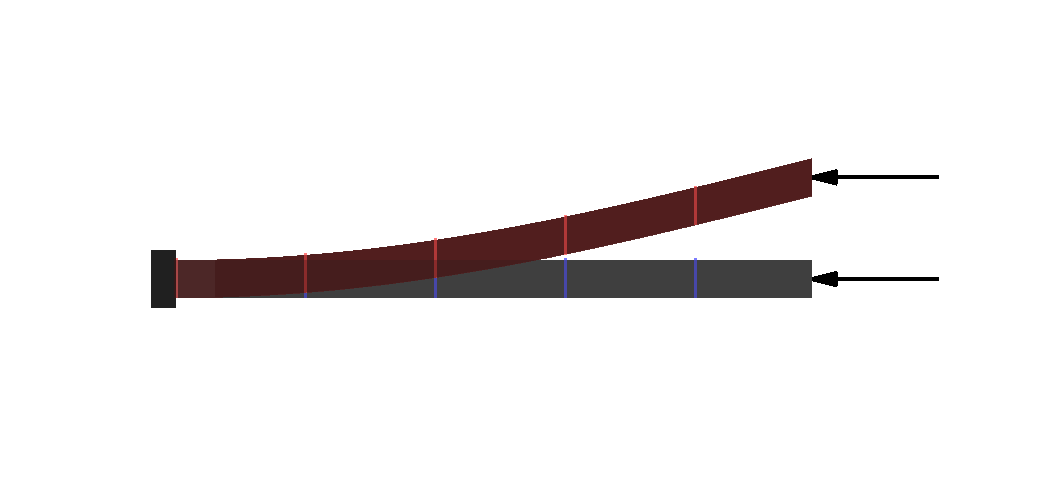
\includegraphics[width=0.49\linewidth]{Cantileverbeam.eps}}
	\subcaptionbox{悬臂梁分岔图\label{fig:Cantileverbeam Bifurcation}}
	{\includegraphics[width=0.49\linewidth]{2_9(2).png}}\\
	\caption{水平压力下的悬臂梁及其分岔图}
	\label{fig:水平压力下悬臂梁的失稳行为}
\end{figure}

下面算例为悬臂梁在非保守力作用下的失稳行为。一长度为$1$,宽厚比为$w/t=10$的悬臂梁,其两个主惯性轴方向的弯曲刚度分别为$0.7097$,$70.9731$,扭转刚度为1,拉伸刚度设为2000,用以约束节点与节点之间的相对距离。将该悬臂梁一端固支,而另一端自由,并在自由端施加跟随力(即压力的作用线方向始终与杆的切线方向保持共线),如图~\ref{fig:Follower Force}所示。当跟随力小于某一临界值时直线构形为稳定构形。当超过该临界值时,直线构形发生动力学失稳,并开始做周期性振荡。

本文结合离散弹性杆模型与COCO的“ep”工具箱求解该结构的平衡解并判断解的稳定性,在压力为$F=14.5$时存在一霍普夫分岔点,该霍普夫分岔点与利用公式\cite{elishakoff2001non}
\begin{equation}
	F_{\mathrm{cr}}=\frac{2\pi^2EI}{L^2}
\end{equation}
求得的理论解$F_{\mathrm{cr}}=14$相吻合。在分岔点之后原平衡构形失稳。另外,当压力$F=15$的情况下,用离散弹性杆进行动力学模拟,可以得到杆在无阻尼的情况下的振荡曲线,如图~\ref{fig:Vibration}。图~\ref{fig:Vibration}中纵坐标为悬臂梁自由端的垂直方向位移,横坐标为时间,在时间小于$1.5$秒时,悬臂梁由于无外界扰动,并未发生振动。但随着数值误差的积累,悬臂梁开始上下振动且振幅不断增大,当时间大于$3$秒时,振幅趋于稳定,悬臂梁此时在稳定的极限环上振动。该动力学模拟验证了结构在霍普夫分岔点之后原直线构形失稳,结构在稳定的极限环上振荡。
\begin{figure}
	\centering
	\subcaptionbox{跟随力作用下的悬臂梁\label{fig:Follower Force}}
	{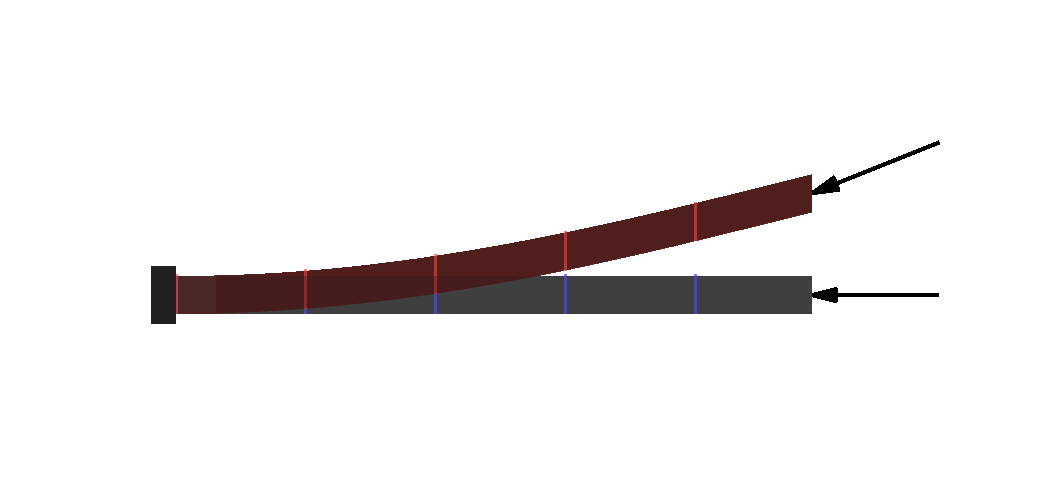
\includegraphics[width=0.49\linewidth]{follower forces.eps}}
	\subcaptionbox{悬臂梁自由端的位置随时间的变化关系\label{fig:Vibration}}
	{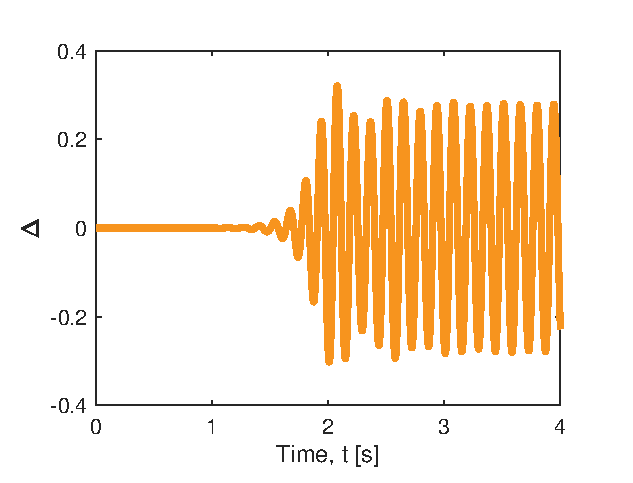
\includegraphics[width=0.49\linewidth]{Vibration.eps}}\\
	\caption{跟随力作用下的悬臂梁及其振动曲线}
	\label{fig:跟随力作用下的悬臂梁的失稳行为}
\end{figure}

通过上述两个算例,说明本文所设计的稳定性判断方法,不仅适用于对静力学稳定性的判断,同时也适用于动力学失稳的判断。
\subsection{剪切条带结构}
本算例中的结构为剪切条带\cite{yu2019bifurcations},其两端固支,长度为$1$。在压力作用下,当压力超过某一临界值时,条带会发生屈曲。继续施加水平压力,直到条带两端之间的距离为$0.5$,形成$\Omega$-型,如图~\ref{fig:Omega strip}所示。在此弯曲的$\Omega$-型上,施加平面外的位移$\Delta Y$,如图~\ref{fig:Sheraband_Shear}所示,结构展现出了复杂的分岔行为。
\begin{figure}
	\centering
	\subcaptionbox{未受载荷下的直线条带\label{fig:straight strip}}
	{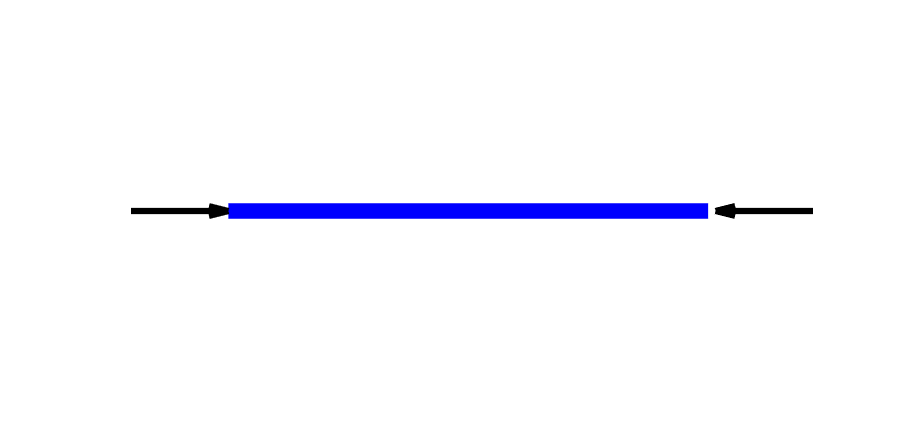
\includegraphics[width=0.49\linewidth]{Shearband_Straight.eps}}
	\subcaptionbox{$\Omega$构形条带\label{fig:Omega strip}}
	{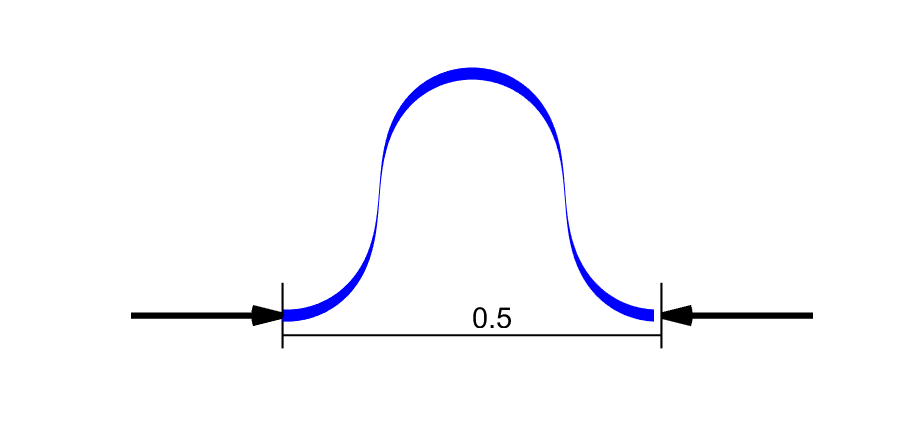
\includegraphics[width=0.49\linewidth]{Shearband_Omega.eps}}\\
	\subcaptionbox{受剪切位移后的条带\label{fig:Sheraband_Shear}}
	{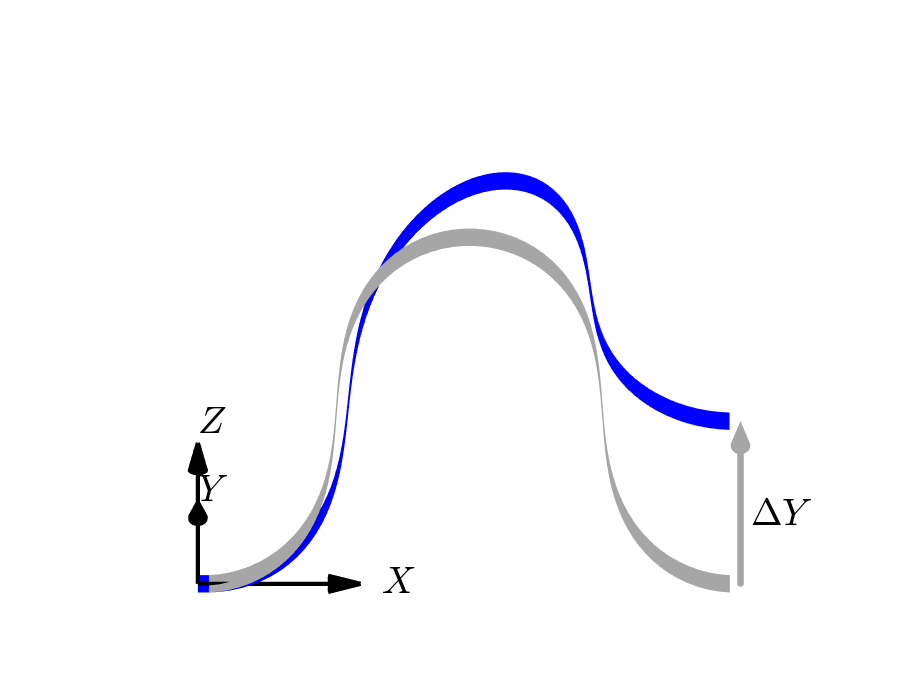
\includegraphics[width=0.7\linewidth]{Shearband_Shear.eps}}
	\caption{不同载荷下的剪切条带}
	\label{fig:不同载荷下的剪切条带}
\end{figure}

本算例中的条带长度为$1$,截面的宽厚比$w/t=20$。其两个主惯性轴方向的弯曲刚度分别为$0.6866$,$274.6550$,扭转刚度为$1$,拉伸刚度设为$2000$,用以约束节点与节点之间的相对距离。在利用离散弹性杆进行计算时,将该条带离散为$100$段。计算中将该弹性条带首端固支,即约束条带首端的两个节点坐标和第一离散段的相对转角;条带末端为滑动支座,即约束最后两个节点非轴向的位移以及最后一段离散弹性杆的相对转角,保持轴向位移自由。随后在末端施加水平方向的压力,当压力值达到$28.035$时,COCO检测到分岔点$BP$以及$SN$点,意味着该压力为条带失稳的临界压力;根据材料力学可知,两端固支的欧拉杆理论临界失稳压力为
\begin{equation}
	F_{\mathrm{cr}}=\frac{4\pi^2EI}{l^2}
\end{equation}
本案例中弯曲刚度为$0.6866$,相应的理论临界压力为$27.1$,与离散弹性杆模型所预测的临界压力相符。在该临界压力处,沿着分支进行延拓,直到压力为$37.565$,此刻条带被压缩为原长的一半,如图~\ref{fig:Omega strip}所示。随后将某端轴向位移的固定,在条带末端施加沿条带宽度的剪切位移$\Delta Y$。
\begin{figure}
	\centering
	\subcaptionbox{剪切条带的分岔图\label{fig:Shearband_Bifurcation}}
	{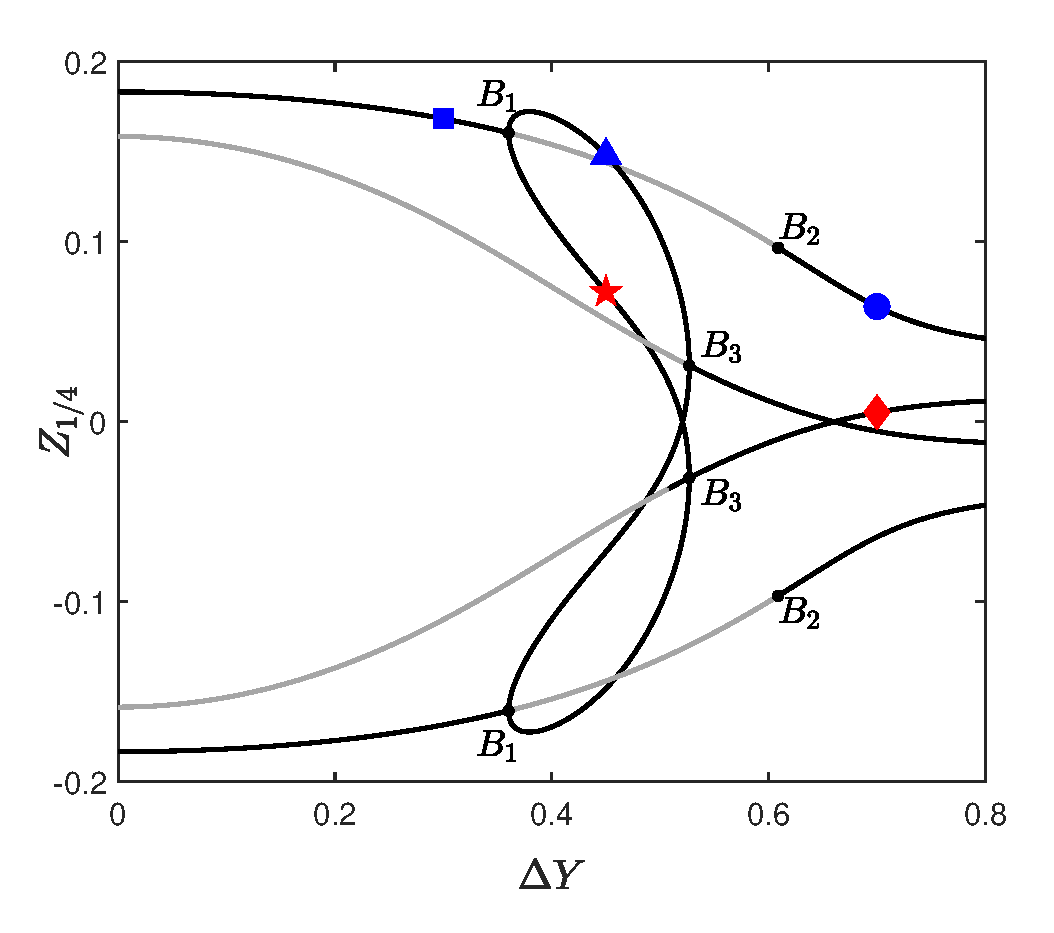
\includegraphics[width=0.8\linewidth]{Shearband_Bifurcation.eps}}\\
	\subcaptionbox{剪切位移为0.36时的稳定构形\label{fig:Shearband_0.36}}
	{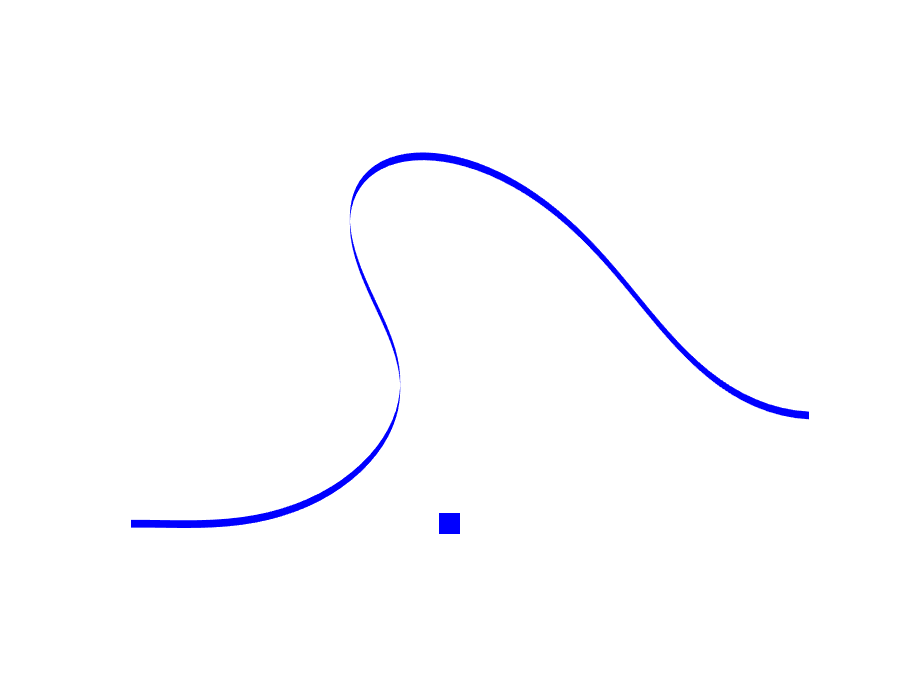
\includegraphics[width=0.3\linewidth]{Shearband_0.36.eps}}
	\subcaptionbox{剪切位移0.45时的稳定构形\label{fig:Shearband_0.45}}
	{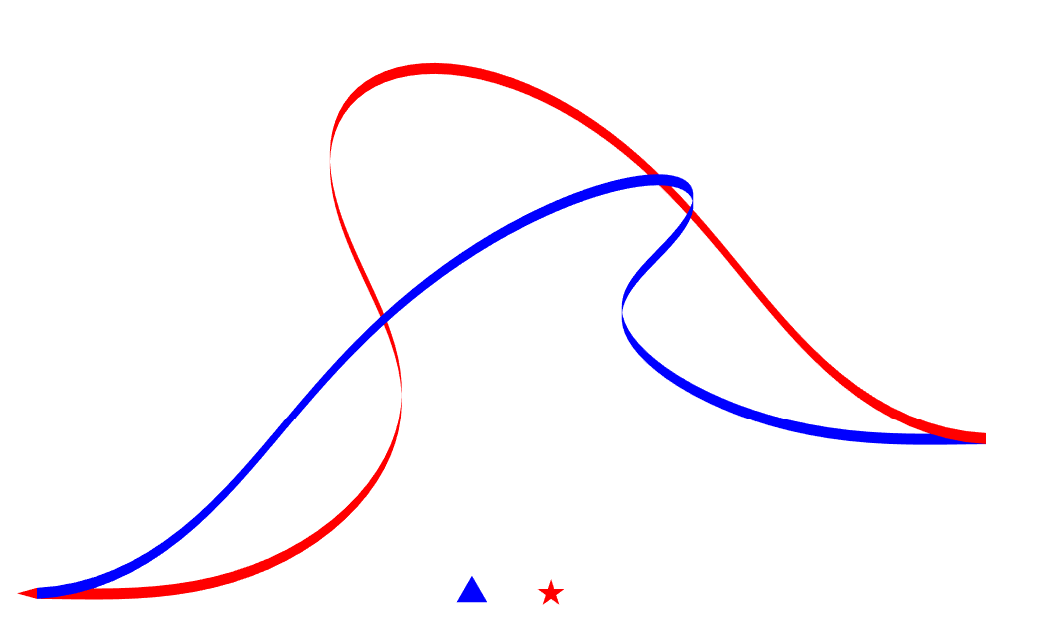
\includegraphics[width=0.3\linewidth]{Shearband_0.45.eps}}
	\subcaptionbox{剪切位移为0.7时的稳定构形\label{fig:Shearband_0.7}}
	{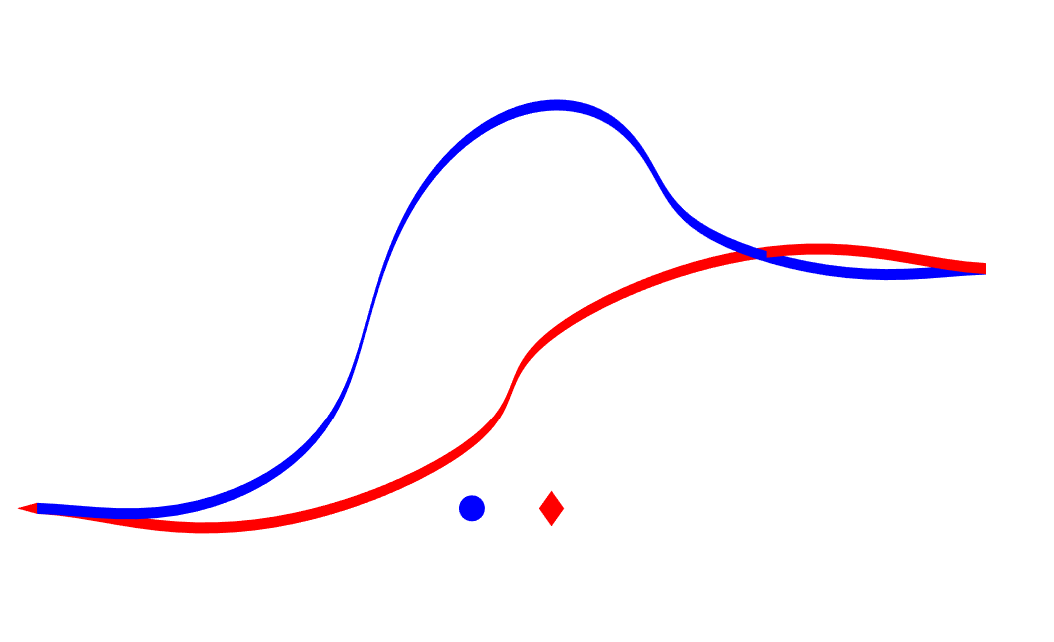
\includegraphics[width=0.3\linewidth]{Shearband_0.7.eps}}
	\caption{剪切条带的分岔图及相应的条带构形}
	\label{fig:剪切条带的分岔图及相应的条带构形}
\end{figure}

图~\ref{fig:Shearband_Bifurcation}为受剪切条带的分岔图,其中横坐标为延拓参数,为沿条带宽度方向($Y$方向)的剪切位移;纵坐标为条带四分之一弧长处的$Z$方向坐标,用于区分不同的平衡分支。以$\Omega$构形为延拓起点,对应图~\ref{fig:Shearband_Bifurcation}中$\Delta Y=0$时的最上侧曲线,当剪切位移逐渐增大并穿过分岔点$B_1$(对应剪切位移为$0.36$)时,同时存在一个SN点,存在一个特征值由负穿过零点变为正,意味着该平衡分支在分岔点$B_1$后失稳。该分支的解在经过分岔点$B_2$(对应剪切位移为$0.608$)时,同时穿过一SN点,存在一个正特征值穿过零点变为负数,该平衡解分支由非稳定状态重新变为稳定状态。从分岔点$B_1$向分支进行延拓,该分支形成一个闭环,整个闭环在延拓过程中无SN点的出现,因此整个分支为稳定解。在分支上存在分岔点$B_3$(对应剪切位移$0.5268$),从该分岔点延拓的分支中,存在一个SN点,将该分支分为稳定部分(剪切位移大于$B_3$)与非稳定部分(剪切位移小于分岔点$B_3$)。图~\ref{fig:Shearband_0.36},~\ref{fig:Shearband_0.45}和图~\ref{fig:Shearband_0.7}展示了部分稳定平衡分支上对应的条带构形,分别对应剪切位移为$0.36$,$0.45$,$0.7$下的稳定平衡构形。

\citet{yu2019bifurcations}利用各向异性杆模型对剪切条带结构进行了分岔分析,并通过实验对其数值计算结果进行了验证。另外,该文章还研究了条带宽厚比对分岔行为的影响。但该文章并未提出一种稳定性判定方法,来验证该结构各个平衡分支的稳定性。本文利用离散弹性杆模型就典型条件(即无宽厚比为$20$)下的剪切条带进行了分岔研究,结果与该文章结果\cite{yu2019bifurcations}吻合很好,包括分岔点位置与各分支解对应的条带构形。另外,本文中使用的稳定性判断准则很好地预测了所有平衡分支的稳定性。该算例说明了本文中提出的稳定性判断准则可以很好地应用于具有复杂分岔行为的结构稳定性判断。
\subsection{发卡结构}
本算例中所研究的结构为类似于图~\ref{fig:hair clips}所示的发卡的双稳态结构,称为Bigon,如图~\ref{fig:bigon}所示。该结构是由两根细长条带在首尾两端相互连接而成的结构。该算例代表了一类多杆系统,比如网状结构\cite{huang2022buckling},多根初始曲率不同的杆依次连接而成的杆件系统\cite{shi2025double}。通过该算例,可以验证本文所提出的稳定性测试方法在复杂杆系统中的适用性与有效性。
\begin{figure}
	\centering
	\subcaptionbox{发卡\label{fig:hair clips}}
	{\includegraphics[width=0.45\linewidth]{发卡.pdf}}
	\subcaptionbox{双条带构成的Bigon结构\cite{yu2021numerical}\label{fig:bigon}}
	{\includegraphics[width=0.45\linewidth]{Bigon图.pdf}}
	\caption{发卡结构与Bigon}
	\label{fig:bigon构形}
\end{figure}

该结构的具体组成过程如图~\ref{fig:Fabrication of Bigon}所示:两根长度为$l$,截面的宽厚比为$w/t=2$的细长杆首末两端固接在一起,两杆端部的切线所构成的夹角为$\gamma$,且首末两端的夹角$\gamma$保持相同。在利用离散弹性杆模型具体计算过程中,两个主惯性轴方向的弯曲刚度分别为$0.9693$,$3.8773$,扭转刚度为$1$,拉伸刚度设为$2000$,用以约束节点与节点之间的相对距离。
\begin{figure}
	\centering
	\includegraphics[width=0.8\linewidth]{Fabrication of Bigon.pdf}
	\caption{Bigon的组装过程\cite{yu2021numerical}}
	\label{fig:Fabrication of Bigon}
\end{figure}

在具体计算过程中,在两细长条带的$0$端,图~\ref{fig:Bigon_First order}所示,施加固支边界条件,即分别固定两杆前两个节点坐标以及第一个离散段上相对转角,该固接边界条件用来固定结构在空间中的位置。另一个端为固接边界条件。考虑到在$\gamma=0^\circ$(两杆处于未变形状态)处,末端两个连接单元构成的离散杆单元具有$180$度的拐角(相邻离散段之间共线且方向相反),根据离散曲率的定义式\eqref{eq:Discrete Curvature}无法定义该状态下的离散曲率因而无法直接利用前文所述的施加固接条件的方法。为此本文在计算过程中,以两杆弯曲为半圆弧时的状态(即$\gamma=180^\circ$)作为参数延拓的起点,延拓过程中逐渐减小角度$\gamma$。
\begin{figure}
	\centering
	\subcaptionbox{一阶屈曲模态\label{fig:Bigon_First order}}
	{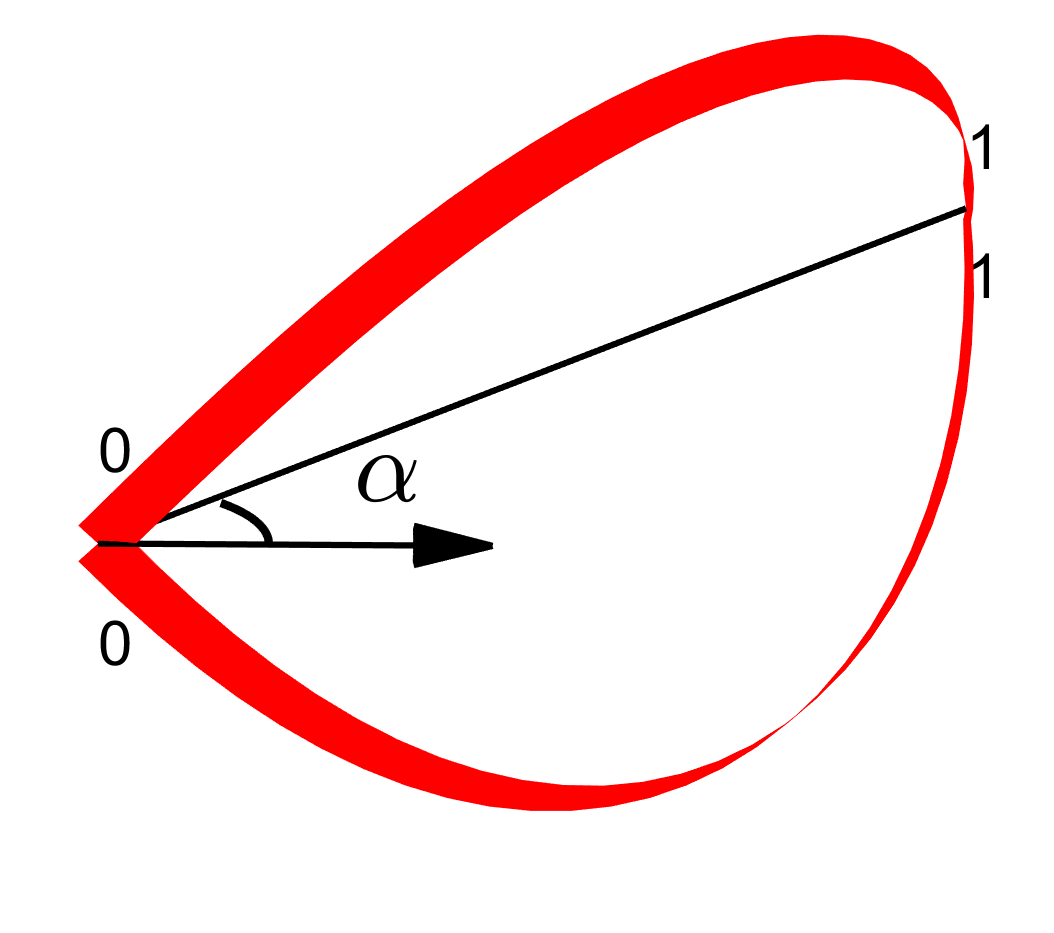
\includegraphics[width=0.4\linewidth]{Bigon_First order.eps}}
	\subcaptionbox{二阶屈曲模态\label{fig:Bigon_Second order}}
	{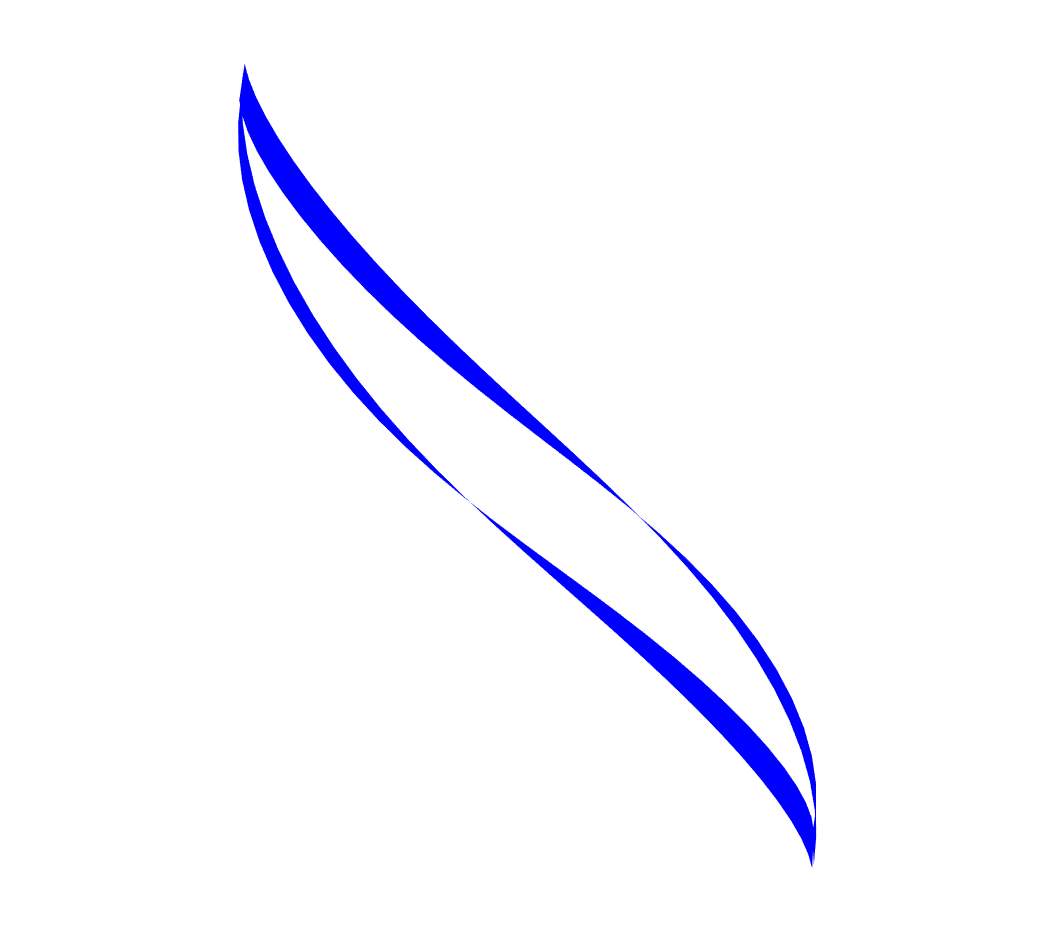
\includegraphics[width=0.4\linewidth]{Bigon_Second_order.eps}}
	\caption{Bigon的一阶屈曲模态与二阶屈曲模态}
	\label{fig:Bigon的一阶屈曲模态与二阶屈曲模态}
\end{figure}
\begin{figure}
	\centering
	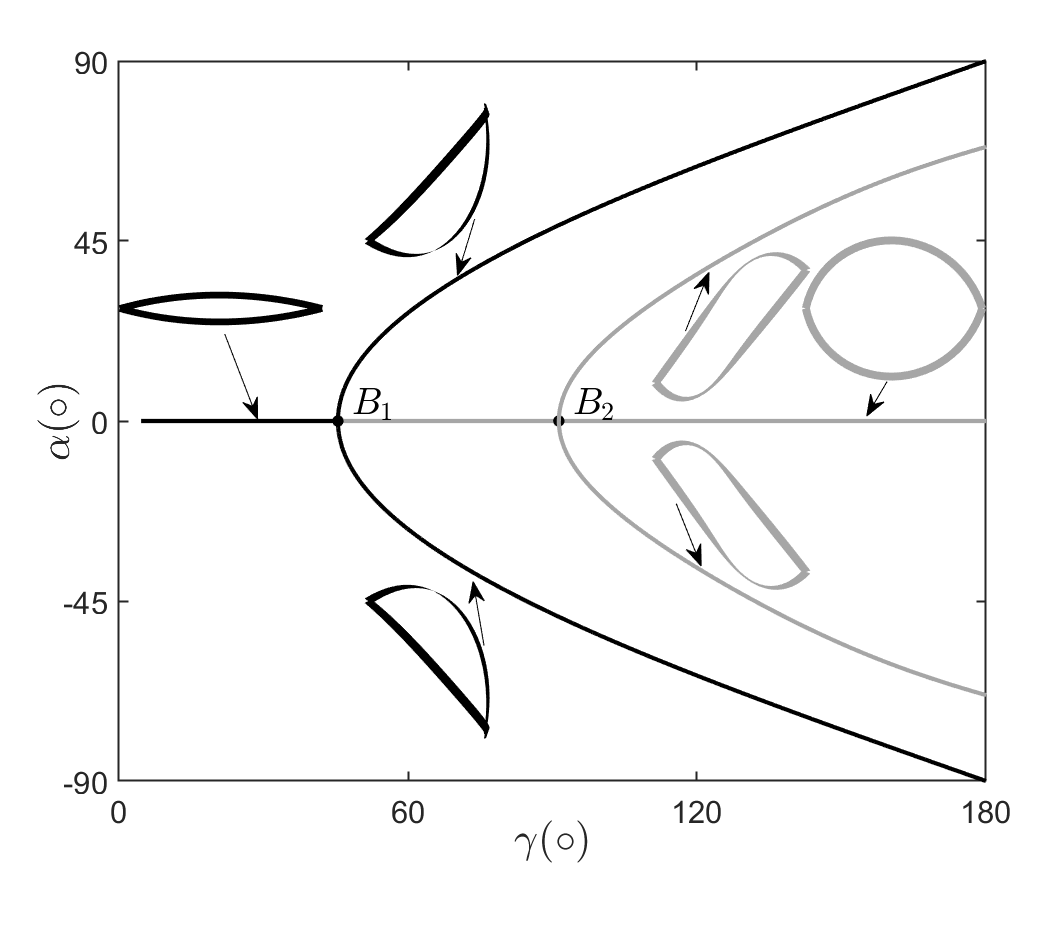
\includegraphics[width=0.7\linewidth]{Bigon_bifurcation.eps}
	\caption{Bigon分岔图}
	\label{fig:Bifurcation digram of Bigon}
\end{figure}

图~\ref{fig:Bifurcation digram of Bigon}展示了bigon的分岔图,其中,延拓参数为$\gamma \in \left[0,180^{\circ} \right]$,即两杆端部切线所构成的夹角。这里通过角度$\alpha$来区分不同的平衡分支,其中$\alpha$是由连接$0$端和$1$端的弦线,与两杆在$0$端的两个切线构成的夹角的角平分线构成的夹角。如图~\ref{fig:Bigon_First order}所示。在分岔图~\ref{fig:Bifurcation digram of Bigon}中横坐标为延拓参数$\gamma$,纵坐标为夹角$\alpha$。在分岔点$B_1$之前(张角$\gamma<45.45^{\circ}$),纵坐标$\alpha$始终保持为零,结构并未发生面外屈曲,保持平面构形,对应图~\ref{fig:Bifurcation digram of Bigon}中最左侧构形。另外,在分岔点$B_1$之前,在任意平衡点处,系统的特征值中无实部为正的特征值,因此该平面构形为稳定构形。当张角$\gamma$超过$B_1$时,结构发生面外屈曲,对应分岔图~\ref{fig:Bifurcation digram of Bigon}中穿过$B_1$的上下对称的平衡分支,平衡分支的对称性是由Bigon本身的对称性决定的,该结构可以向平面外任意一侧弯曲,其屈曲构形为图~\ref{fig:Bifurcation digram of Bigon}中两个上下对称的黑色构形,该构形为结构的一阶屈曲模态,如图~\ref{fig:Bigon_First order}所示。而其在分岔点$B_1$之后分岔点$B_2$之前($45.45^{\circ}<\gamma<91.3176^{\circ}$)的平面平衡解中,系统存在一个具有正实部的特征值,因此,平面解变为不稳定解,用灰色直线表示。而屈曲构形对应的平衡解的特征值中无实部为正的特征值,因此为稳定解。而在分岔点$B_2$之后,平面平衡解对应的特征值中有三个实部为正的特征值,平面解仍为非稳定解。二阶屈曲模态为不稳定构形,如图~\ref{fig:Bigon_Second order}所示,对应图中经过$B_2$的上下对称的不稳定分支。

Yu等\cite{yu2021numerical}利用基尔霍夫杆模型对该结构进行了分岔分析,并利用实验的手段对各个平衡解进行了稳定性判断。但并未通过数值的手段给出该结构平衡解的稳定性信息。本文中利用离散弹性杆模型结合分岔分析工具包COCO,对该结构进行了分岔分析并对所得平衡解进行稳定性判断。本文结果(包含分岔点位置以及稳定性判断结果)与Yu等\cite{yu2021numerical}的结果吻合良好,说明了该稳定性判断方法对多杆结构的有效性。
